% Asset ID: FA22SamplingAndEstimationTikZ-002
% Asset type: TikZ diagram
% Topic code: FA22-EST
% Purpose: Confidence interval number line with xbar, margin of error and width.
\documentclass[tikz,border=8pt]{standalone}
\usepackage{amsmath}
\usepackage{xcolor}
\usetikzlibrary{arrows.meta,decorations.pathreplacing}
\definecolor{Canvas}{HTML}{FAF9F6}\definecolor{Ivory}{HTML}{FFFFF0}\definecolor{LineSoft}{HTML}{E5E5EA}\definecolor{Gold}{HTML}{C5A059}\definecolor{GoldDeep}{HTML}{D4AF37}\definecolor{Blush}{HTML}{FBEFEF}\definecolor{Ink}{HTML}{2C2C2E}
\begin{document}
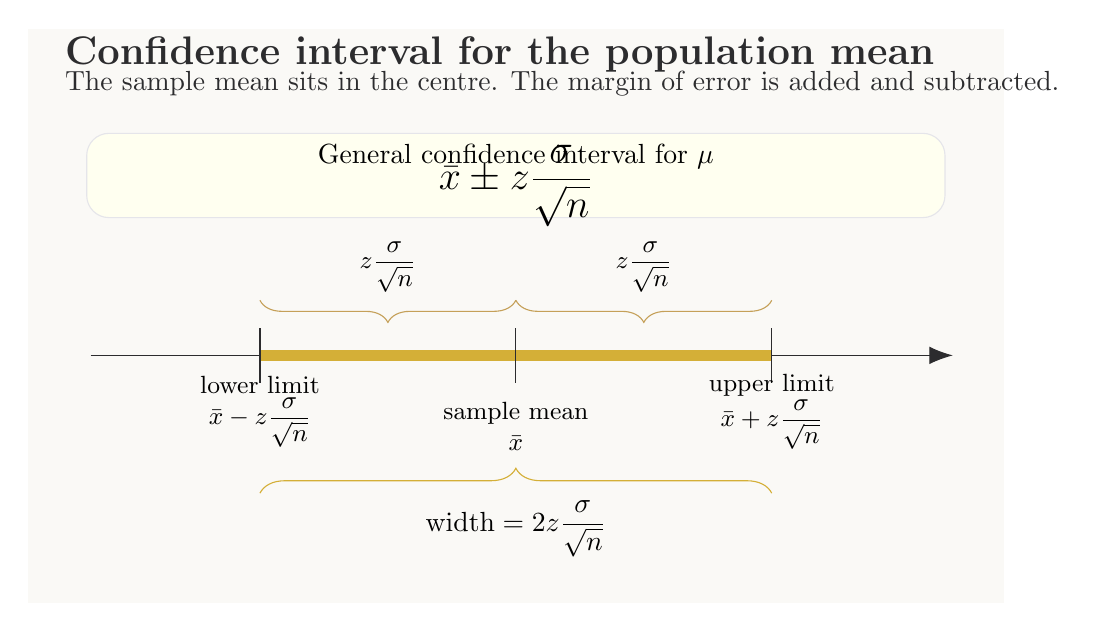
\begin{tikzpicture}[x=1cm,y=1cm]
\fill[Canvas] (-6.2,-3.15) rectangle (6.2,4.15);
\node[anchor=west, text=Ink, font=\bfseries\Large] at (-5.85,3.82){Confidence interval for the population mean};
\node[anchor=west, text=Ink] at (-5.85,3.45){The sample mean sits in the centre. The margin of error is added and subtracted.};
\draw[Ink, -{Latex[length=3mm]}] (-5.4,0) -- (5.55,0);
\coordinate (L) at (-3.25,0);\coordinate (C) at (0,0);\coordinate (U) at (3.25,0);
\draw[GoldDeep, line width=4pt] (L) -- (U);
\foreach \p in {L,C,U}{\draw[Ink] (\p) -- ++(0,0.35);\draw[Ink] (\p) -- ++(0,-0.35);}
\node[align=center,font=\small] at (-3.25,-0.72){lower limit\\\(\displaystyle \bar{x}-z\frac{\sigma}{\sqrt{n}}\)};
\node[align=center,font=\small] at (0,-0.9){sample mean\\\(\displaystyle \bar{x}\)};
\node[align=center,font=\small] at (3.25,-0.72){upper limit\\\(\displaystyle \bar{x}+z\frac{\sigma}{\sqrt{n}}\)};
\draw[decorate,decoration={brace,amplitude=8pt,mirror},Gold] (-3.25,0.7)--(0,0.7);
\node[font=\small] at (-1.625,1.12){\(\displaystyle z\frac{\sigma}{\sqrt n}\)};
\draw[decorate,decoration={brace,amplitude=8pt,mirror},Gold] (0,0.7)--(3.25,0.7);
\node[font=\small] at (1.625,1.12){\(\displaystyle z\frac{\sigma}{\sqrt n}\)};
\draw[decorate,decoration={brace,amplitude=9pt},GoldDeep] (-3.25,-1.75)--(3.25,-1.75);
\node at (0,-2.2){\(\displaystyle \text{width}=2z\frac{\sigma}{\sqrt n}\)};
\draw[LineSoft, rounded corners=8pt, fill=Ivory] (-5.45,1.75) rectangle (5.45,2.82);
\node at (0,2.52){General confidence interval for \(\mu\)};
\node[font=\Large] at (0,2.15){\(\displaystyle \bar{x}\pm z\frac{\sigma}{\sqrt n}\)};
\end{tikzpicture}
\end{document}
